
\chapter{The Comordo recommender system}\label{cha:recsys}

This chapter describes the background of the thesis and the task given by given by Comordo for the construction of the recommender system which is the main purpose of the thesis from Comordo's point of view. Then a rundown of mathematical theory of the used recommendation model and description of the used algorithms follow.

%Then background theory about supervised learning, the used recommendation model and evaluating recommendations and a summary of optimization strategies are given.  Descriptions of the algorithms \textit{katz-eig} and \textit{link-analysis} follow.

Comordo Technologies is a startup in recommendation systems driven inside the bounds of LiU's incubator LEAD in Linköping and will in the future offer a cloud service for e-commerce. The base for the recommendation system is algorithms based on predication and machine learning. At the start of this thesis the company stood to build a first version of it's recommendation system.

Comordo focuses on generating personal recommendations using \textit{implicit feedback} aimed at e-commerce using purchase history for users as their main focus. The end product aims to be a remote API where e-commerce clients queries for precomputed recommendations made for their users.

\Warning[TODO]{ Stich together }

This chapter presents the development methodology used, then the datasets used and finally the evaluation method for evaluating recommendation quality are presented.

The thesis can be split in two major parts. A system development part where a first version of Commordo's recommender system is built, the ``glue'' around the recommender algorithms. The second part with development of a learning framework for the algorithms and an analysis of the algorithms' parameters.

The focus on the beginning is on the system development part and with that in place the focus shiftes to the learning framework and parameter tuning.

\section{Development methodology}

The software development side of the thesis

\textit{Agile, iterative etc...}

The software will be developed using agile inspired methods. Iterative development will be used to produce a simple prototype and then iteratively improve and add more features. The early priority is to produce a working chain from reading data to storing recommendations in the database.

Small incremental goals will be used, an example goal could be to complete a reader plugin for a specific dataset.

Automatic tests shall be used but not in the test driven development way.


\subsection{Programming languages}

Why matlab? Why python? Why not something else? (Julia, numpy, scipy, C, C++, ...)?

The existing algorithms exists in a prototype form in Matlab. The thesis will continue to use the algorithms written in Matlab for easy prototyping and modifications. Python will be used as glue and be used to implement all modules (see \sectionref{sec:sysoverview}).

Using other languages or platforms, such as Julia, C, C++, or Python with NumPy or SciPy could give performance improvements, but it's not in the scope of this thesis. Also as Comordo is in it's startup phase with focus on prototyping it is valuable to continue with a platform familiar to them.



\section{Evaluation}\label{sec:method:eval}

Recommendation quality was evaluated using \textit{Precision}, \textit{Recall} and \textit{F-measure} with top-10 recommendations. Focus was on \textit{F-measure} as a combined measure of \textit{Precision} and \textit{Recall}.

The following steps describes the steps taken to produce evaluations given the training, validation and test sets $A_{train}$, $A_{val}$ and $A_{test}$:

\begin{enumerate}
    \item Produce recommendation predictions $p_{u, i}$ from $A_{train}$ with the chosen algorithm.
    \item Transform $p_{u, i}$ to a set of binary recommendations $r_{u, i}$ using the top-10 most predicted items for each user, by the process described in \chapterref{cha:theory}.
    \item Evaluate \textit{F-measure}, as described in \sectionref{sec:background:theory:eval}, with $e_{u, i}$ representing $A_{val}$ or $A_{test}$, depending on which set to evaluate against.
\end{enumerate}

If not explicitly noted, the evaluation set was the test set.




\section{Use case}\label{sec:use}

\begin{enumerate}
    \item Purchase history and product data is provided by e-commerce clients and consumed by the recommender system.
    \item Load algorithms with purchase history and is run on a nightly basis.
    \item Repopulate recommendation database with new recommendations.
    \item Final customers visit the e-commerce website and are given recommendations delivered to the website via Commordo's remote API.
\end{enumerate}


\section{System overview}\label{sec:sysoverview}

Figure \ref{fig:sysoverview} is a sketch of Commordo's recommender system, as planned for at the start of the thesis.

\begin{figure}[h!]
  \centering
    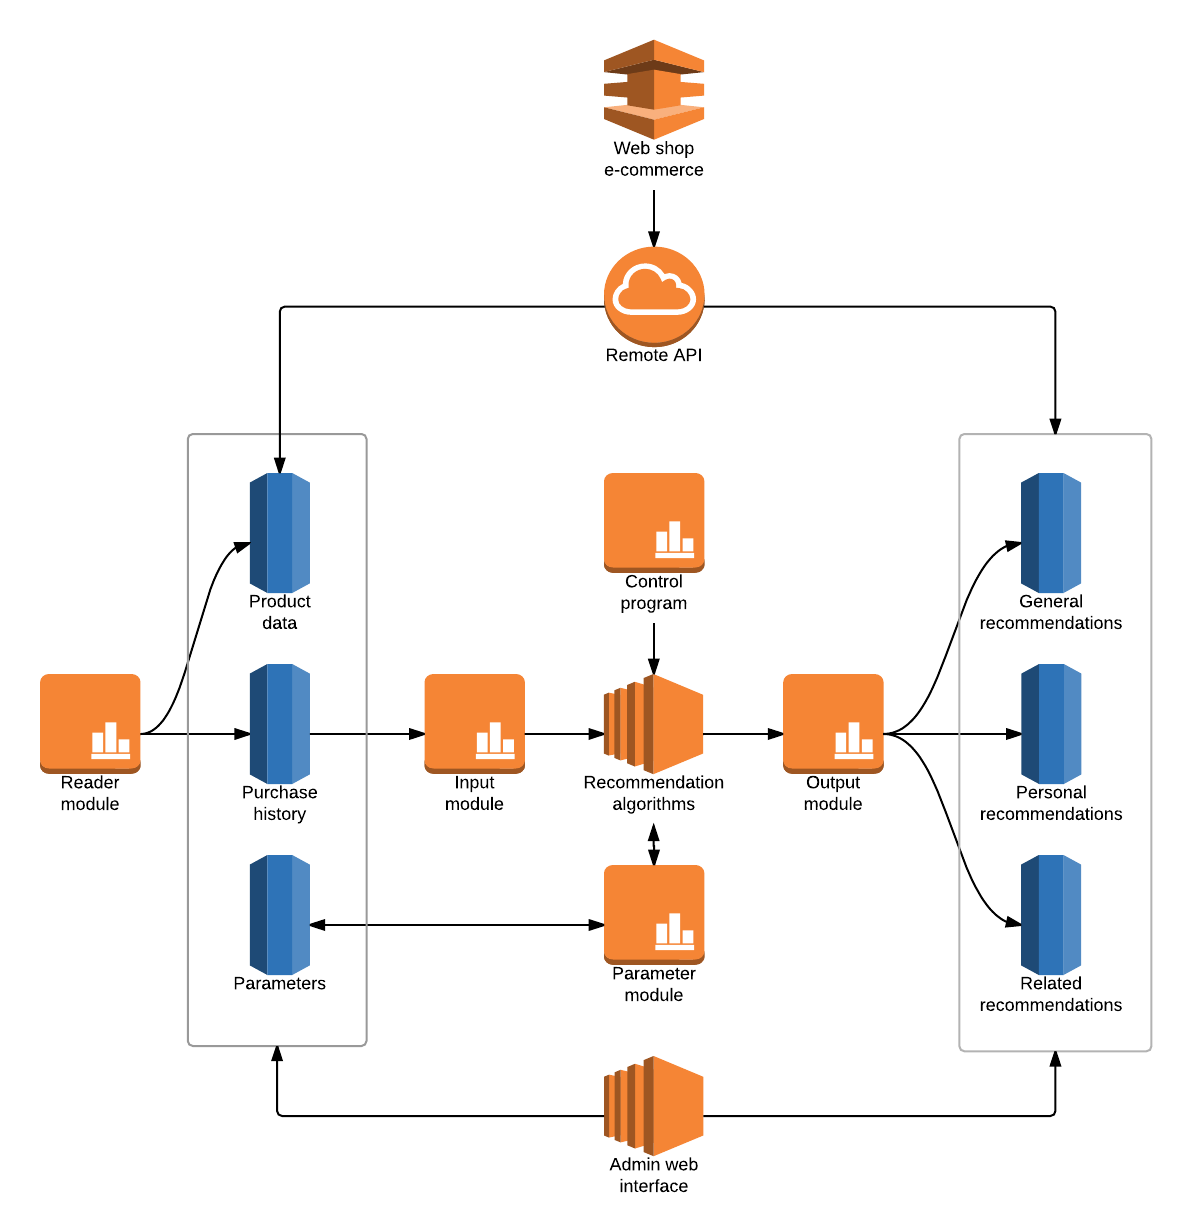
\includegraphics[width=0.9\textwidth]{fig/system_overview.png}
  \caption{Commordo's system sketch}
  \label{fig:sysoverview}
\end{figure}

\FloatBarrier

\begin{description}
    \item[Reader module] is responsible for reading data files provided by Commordo's clients.
    \item[Input module] provides the algorithms with transformed data.
    \item[Output module] populates the database with recommendations.
    \item[Control program] handles learning and optimization of the algorithms.
    \item[Parameter module] stores and adjusts parameters the algorithms use.
    \item[Remote API] is a REST based API, the endpoint for Commordo's clients.
    \item[Admin web interface] is a user friendly way for e-commerce clients to customize system settings and view recommendations.
\end{description}



\section{Task}\label{sec:task}

The task for this thesis was to complete the backend of Commordo's system. This includeded the reader, input, output and parameter modules, the storage of purchase history and parameters and algorithms for parameter tuning. The other databases were be provided, but with some level of adaptation. The recommender algorithms were given. The admin interface and the remote API are not included in this thesis.




\section{System overview}\label{sec:res:sys}

Describe the system as a whole here, and what parts have been done.

\begin{enumerate}
    \item Reader module (inläsningsmodul, name????)
    \item Input module (indata) name???
    \item Output module (utdata)
    \item Purchase history db
    \item Product data db
    \item Parameters??? Or will we ignore this for the thesis work?
    \item Algorithm
    \item Control programs (But it's really just modifications of the algorithms)
    \item General/Personalized/Related recommendations db
    \item Remote API
    \item Web shop
    \item Admin web API?
\end{enumerate}

\Warning[TODO]{ Need a figure which describes the different parts }


\subsection{Input module}\label{sec:res:input}

Describe plugin based architecture here.

Add plugin scripts to:


\begin{lstlisting}
    lib/reader_plugins
\end{lstlisting}

Basic look is:

% TODO include files instead, or delegate to appendix?
\begin{lstlisting}[language=python]
class MyPlugin():

    def add_arguments(self, parser):
        """Parse command line arguments"""

        parser.description = "Load plugin data"

        parser.add_argument('data_file', metavar='data_file', type=str,
                            help='the file to parse')

    def load(self, args):
        """Load users and products."""

        products = {}
        users = {}

        # Parse data file
        with open(args.data_file) as csvfile:
            reader = csv.DictReader(csvfile, delimiter=';', quoting=csv.QUOTE_NONE)

            for row in reader:
                user_id = row['shopper_id']
                isbn = row['isbn']
                title = row['description']

                if user_id not in users:
                    users[user_id] = User(user_id)

                if isbn not in products:
                    product = Product(isbn)
                    product.isbn = isbn
                    product.title = title
                    products[isbn] = product

                users[user_id].add_history(isbn, 1)

        return users, products
\end{lstlisting}

An example plugin is described in appendix X. \Warning[TODO]{ Make it happen! }

Can describe how to dynamically locate modules with python, but that's not the purpose is it? Just describe that it can be done I guess?




\section{Data}

The available datasets are described in detail in \appendixref{cha:datasets}. All data will in unweighted binary form \eqref{eq:hist}.

An alternative to unweighted binary data is weighted data, where $h_{u, i} = x$ means that user $u$ has interacted with item $i$ $x$ times. There is some support in the available datasets (\textit{alpha}, \textit{alpha2}) but most of the datasets does not, which is why the focus is on datasets in unweighted binary form.

Another popular format is ratings, which \textit{movielens1m} is derived from. Generating recommendations with explicit feedback, such as ratings, is well researched but fundamentally different from implicit feedback systems. The focus on this thesis is recommendations for implicit feedback systems which is why ratings are not considered in their raw form.

During supervised learning the datasets will be divided into training, validation and test sets with a ratio of 70\%, 15\% and 15\% respectively. When a validation set is not necessary, it will be ignored and only the training and test sets will be used. Alternatively a new split with only training and test sets could be used with, for example, a split of 80\% and 20\% could be used. This thesis uses the same approach because of simplicity, there's no need to track different kinds of splits for the same data.

As mentioned in \sectionref{sec:background:theory:suplearn} there are different ratios commonly used to split datasets. There is no ratio which is always the best, they depend on the amount of data available, the modeled domain and the algorithms chosen. A split of 70/15/15 was chosen uniformly for simplicity reasons.





\newpage
